\documentclass[tikz,border=3pt]{standalone}
\usepackage[T1]{fontenc}
\usepackage{amsmath}\usepackage{graphicx}
\usepackage{XCharter}
\usepackage[xcharter]{newtxmath}
\usepackage[scaled=.92]{helvet}
\usepackage{pgfplots}
\usetikzlibrary{arrows.meta,positioning,fit,calc,backgrounds,decorations.pathreplacing,patterns}
\usepgfplotslibrary{groupplots,fillbetween}
\pgfplotsset{compat=1.18}
\definecolor{ink}{HTML}{172536}
\definecolor{rgb}{HTML}{3563B8}
\definecolor{event}{HTML}{17857C}
\definecolor{fusion}{HTML}{76529C}
\definecolor{reference}{HTML}{8994A3}
\definecolor{warn}{HTML}{AC5948}
\definecolor{muted}{HTML}{657183}
\definecolor{rule}{HTML}{D9E0E8}
\definecolor{pale}{HTML}{F5F7FA}
\color{ink}
\tikzset{box/.style={rounded corners=2pt,draw=rule,fill=white,align=center,inner sep=4pt,font=\sffamily\fontsize{9}{10.8}\selectfont,minimum height=9mm},rb/.style={box,draw=rgb!50,fill=rgb!5},eb/.style={box,draw=event!50,fill=event!5},fb/.style={box,draw=fusion!55,fill=fusion!5},arrow/.style={-{Latex[length=1.8mm]},line width=.65pt,draw=muted},note/.style={font=\sffamily\fontsize{8.4}{10.2}\selectfont,align=center,text=muted},heading/.style={font=\sffamily\fontsize{10}{12}\selectfont\bfseries,align=left,text=ink}}
\pgfplotsset{paper/.style={width=15.7cm,height=6cm,axis lines*=left,axis line style={rule},tick style={draw=none},tick label style={font=\sffamily\fontsize{8.8}{10.4}\selectfont,text=muted},label style={font=\sffamily\fontsize{9.4}{11}\selectfont,text=ink},title style={font=\sffamily\fontsize{10}{12}\selectfont\bfseries,text=ink},legend style={draw=none,fill=none,font=\sffamily\fontsize{9}{11}\selectfont,cells={anchor=west}},grid=major,grid style={rule!65,line width=.3pt},minor tick num=0,scaled ticks=false,unbounded coords=jump,clip mode=individual}}

\hyphenpenalty=10000\exhyphenpenalty=10000
\tikzset{box/.append style={font=\sffamily\fontsize{8}{10}\selectfont},
note/.append style={font=\sffamily\fontsize{8}{10}\selectfont}}
% Generated by scripts/make_official_results.py; do not edit by hand.
\providecommand{\OfficialPhasePublishedOverallMiD}{35.80}
\providecommand{\OfficialOverallAbsoluteGain}{9.228548419}
\providecommand{\OfficialBandContributionSubtotal}{9.227548419}
\providecommand{\OfficialDisplayRoundingResidual}{0.0010}
\providecommand{\OfficialCrucialSmallContributionShare}{82.4\%}
\providecommand{\OfficialPhaseOverallMiD}{35.8015}
\providecommand{\OfficialGarlOverallMiD}{45.03}
\providecommand{\OfficialOverallRelativeGain}{20.49\%}
\providecommand{\OfficialPhaseCrucialMiD}{43.5190}
\providecommand{\OfficialGarlCrucialMiD}{53.13}
\providecommand{\OfficialCrucialRelativeGain}{18.09\%}
\providecommand{\OfficialPhaseSmallMiD}{28.2568}
\providecommand{\OfficialGarlSmallMiD}{37.58}
\providecommand{\OfficialSmallRelativeGain}{24.81\%}
\providecommand{\OfficialPhaseLargeMiD}{25.7179}
\providecommand{\OfficialGarlLargeMiD}{40.61}
\providecommand{\OfficialLargeRelativeGain}{36.67\%}
\providecommand{\OfficialPhaseNegativeMiD}{29.9314}
\providecommand{\OfficialGarlNegativeMiD}{31.29}
\providecommand{\OfficialNegativeRelativeGain}{4.34\%}
\providecommand{\OfficialSampleCount}{6,762}
\providecommand{\OfficialPhaseFailureRate}{0.0\%}
\providecommand{\OfficialGarlFailureRate}{0.0\%}
\providecommand{\OfficialPhaseSubmissionID}{1016512}
\providecommand{\OfficialGarlSubmissionID}{817519}

\begin{document}

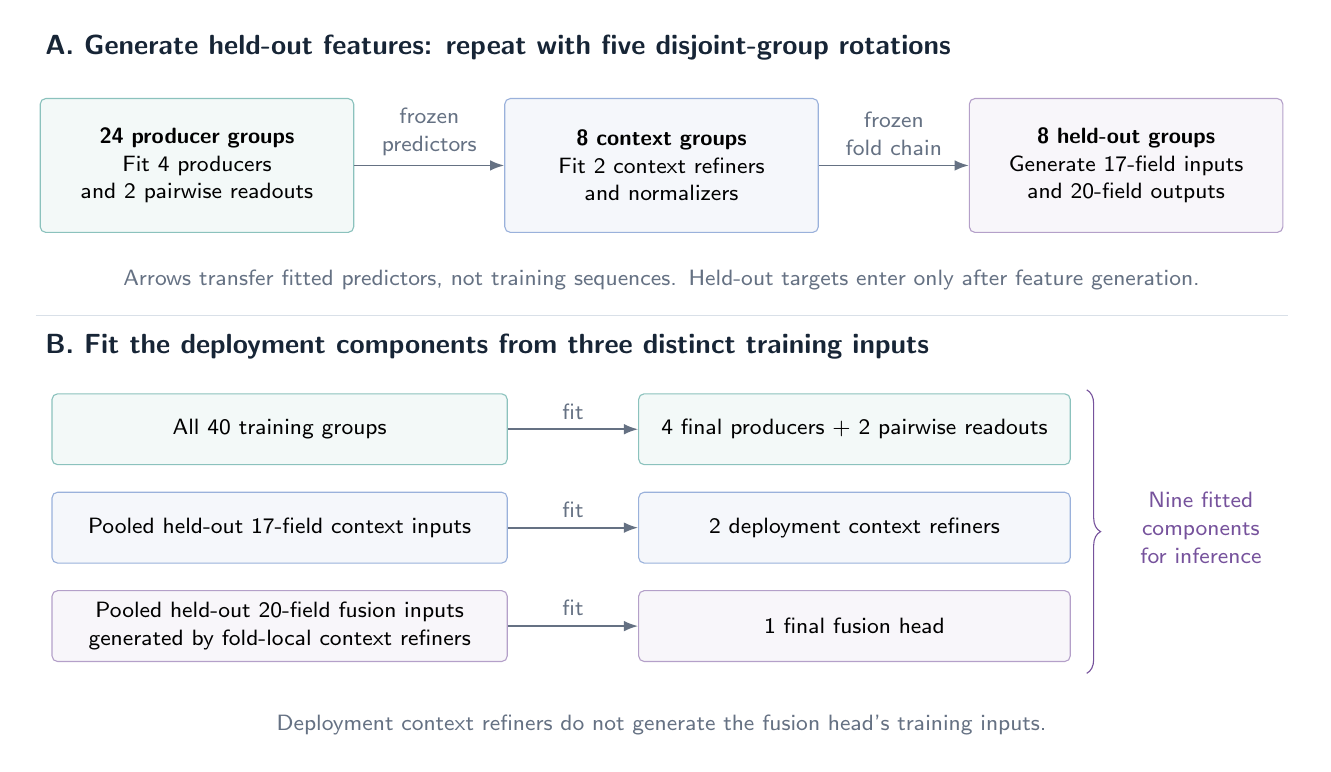
\begin{tikzpicture}[x=1cm,y=1cm]
\path[use as bounding box] (0,-.2) rectangle (16.2,8.9);
\node[heading,anchor=west] at (.1,8.65) {A. Generate held-out features: repeat with five disjoint-group rotations};
\node[eb,text width=3.7cm,minimum height=17mm] (p) at (2.15,7.15) {\textbf{24 producer groups}\\Fit 4 producers\\and 2 pairwise readouts};
\node[rb,text width=3.7cm,minimum height=17mm] (c) at (8.05,7.15) {\textbf{8 context groups}\\Fit 2 context refiners\\and normalizers};
\node[fb,text width=3.7cm,minimum height=17mm] (v) at (13.95,7.15) {\textbf{8 held-out groups}\\Generate 17-field inputs\\and 20-field outputs};
\draw[arrow] (p.east)--node[above,note,text width=1.7cm]{frozen\\predictors}(c.west);
\draw[arrow] (c.east)--node[above,note,text width=1.7cm]{frozen\\fold chain}(v.west);
\node[note,text width=15.7cm] at (8.05,5.7) {Arrows transfer fitted predictors, not training sequences. Held-out targets enter only after feature generation.};
\draw[rule] (.1,5.25)--(16,5.25);
\node[heading,anchor=west] at (.1,4.85) {B. Fit the deployment components from three distinct training inputs};
\node[eb,text width=5.5cm] (data) at (3.2,3.8) {All 40 training groups};
\node[eb,text width=5.2cm] (prod) at (10.5,3.8) {4 final producers + 2 pairwise readouts};
\node[rb,text width=5.5cm] (seventeen) at (3.2,2.55) {Pooled held-out 17-field context inputs};
\node[rb,text width=5.2cm] (ctx) at (10.5,2.55) {2 deployment context refiners};
\node[fb,text width=5.5cm] (twenty) at (3.2,1.3) {Pooled held-out 20-field fusion inputs\\generated by fold-local context refiners};
\node[fb,text width=5.2cm] (fuse) at (10.5,1.3) {1 final fusion head};
\draw[arrow] (data)--node[above,note]{fit}(prod);
\draw[arrow] (seventeen)--node[above,note]{fit}(ctx);
\draw[arrow] (twenty)--node[above,note]{fit}(fuse);
\draw[decorate,decoration={brace,amplitude=5pt},fusion] (13.45,4.3)--(13.45,.7);
\node[note,text width=2cm,text=fusion] at (14.9,2.55) {Nine fitted\\components\\for inference};
\node[note,text width=15.8cm] at (8.05,.05) {Deployment context refiners do not generate the fusion head's training inputs.};
\end{tikzpicture}
\end{document}
